% вторая часть

\section{Разработка микродрона}
\subsection{Разработка архитектуры микродрона}
\subsection{Компоненты квадрокоптера}

Набор наземной станции и квадрокоптера в основном планируется использовать в помещении. В случае использования БПЛА на улице, при весе свыше 250г требуется регистрация, согласно воздушному кодексу Российской Федерации \cite{ivp}. Основываясь на этом, поставлены следующие условия к компонентам квадрокоптера:
\begin{itemize}
	\item размер не должен превышать 140*140*50 \(мм^3\);
	\item полетный вес должен быть ниже 250 г;
	\item квадрокоптер должен выдерживать столкновения;
	\item пропеллеры должны быть защищены;
	\item обеспечена безопасность для детей;
	\item минимальное полетное время 5 мин;
	\item возможность обмениваться телеметрией.
\end{itemize}
В ходе проведения анализа рынка радиоуправляемых квадрокоптеров было выявлено, что готовых вариантов, соответствующих вышеперечисленным условиям, нет. В связи с чем необходимо подобрать компоненты и собрать вручную.

Подходя к вопросу выбора рамы, стоит учитывать такие факторы как:
\begin{itemize}
	\item прочность рамы;
	\item легкий вес;
	\item диагональную жесткость;
	\item стоимость;
	\item расстояния между отверстиями, совпадающие с монтажными отверстиями на электронике.
\end{itemize}
Диагональная жесткость важна для уменьшения собственной частоты колебаний рамы. Чем меньше собственная частота колебаний, тем больше фильтрации требуется, чтобы не вносить в гироскоп осцилляции, которые ухудшают работу ПИД регулятора полетного контроллера. Использование излишней фильтрации приведет к ПИД осцилляциям.

Были проведены испытания с рамами из разных материалов. Рассматривались следующие альтернативы: фанера, PLA, PETG и угольно -- армированный пластики, текстолит и углепластик (композитный пластик, также известный как карбон). Фанера обладает низкой стоимостью, но уступает по жесткости остальным альтернативам. PLA пластик самый безопасный для здоровья человека, им можно печатать детали на 3d принтере, но не устойчив к ударам. PETG обладает большей прочностью по сравнению с PLA, но недостаточно жесткий, в связи с чем уменьшается собственная частота колебаний. Угольно-армированный пластик позволяет обеспечить жесткость и прочность рамы, но является одним из самых дорогих вариантов и обусловлен трудностями печати.
Текстолит является самым жестким среди вышеперечисленных альтернатив, но обладает самым большим весом. Композитный пластик на основе карбонового волокна самый дорогой из перечисленных, однако является самым прочным, жестким и относительно легким вариантом. Таким образом, было решено использовать карбоновую раму.
Защита для пропеллеров пластиковая, так как обладает упругостью и низкой стоимостью.

Форм фактор рамы также является немаловажной деталью. Для выполнения задач позиционирования и навигации в зависимости от условий необходимо будет поворачивать камеру вниз, вперед и вверх. Исходя из этого, необходимо, чтобы защита пропеллеров, пластины рамы, а также аккумулятор не перекрывали обзор/уменьшали область видимости. Оптимальным решением является рама с вытянутым корпусом и расположением лучей по типу deadcat -- передние лучи разведены на угол, близкий к 180 градусам. Расстояние между отверстиями для монтажа электроники выгоднее выбирать из стандартов -- 16*16, 20*20 или 25,5*25,5 мм. Вариант 25,5*25,5мм рассматривать стоит только в том случае, если необходимо использовать “все в одном”: плату, совмещающую полетный контроллер и регуляторы в одном устройстве. Для поставленной цели -- создания учебного набора квадрокоптера такая плата неуместна по следующим причинам:
\begin{itemize}
	\item в случае поломки заменяется полностью;
	\item стоимость выше, чем у комплекта раздельных регуляторов и полетного контроллера;
	\item выбор такого формата плат, с ресурсами, необходимыми для реализации проекта, крайне мал.
\end{itemize}
Основываясь на вышеперечисленном была приобретена рама, представленная на рисунке \ref{fig:frame}. Она позволяет установить нано камеру (размером 14*14 мм), стеки из полетного контроллера и регуляторов с посадочными отверстиями 20x20mm/16x16mm, моторы размера 1102-1308 и пропеллеры диаметром до 40 мм.

\begin{figure}[H]
	\centering
	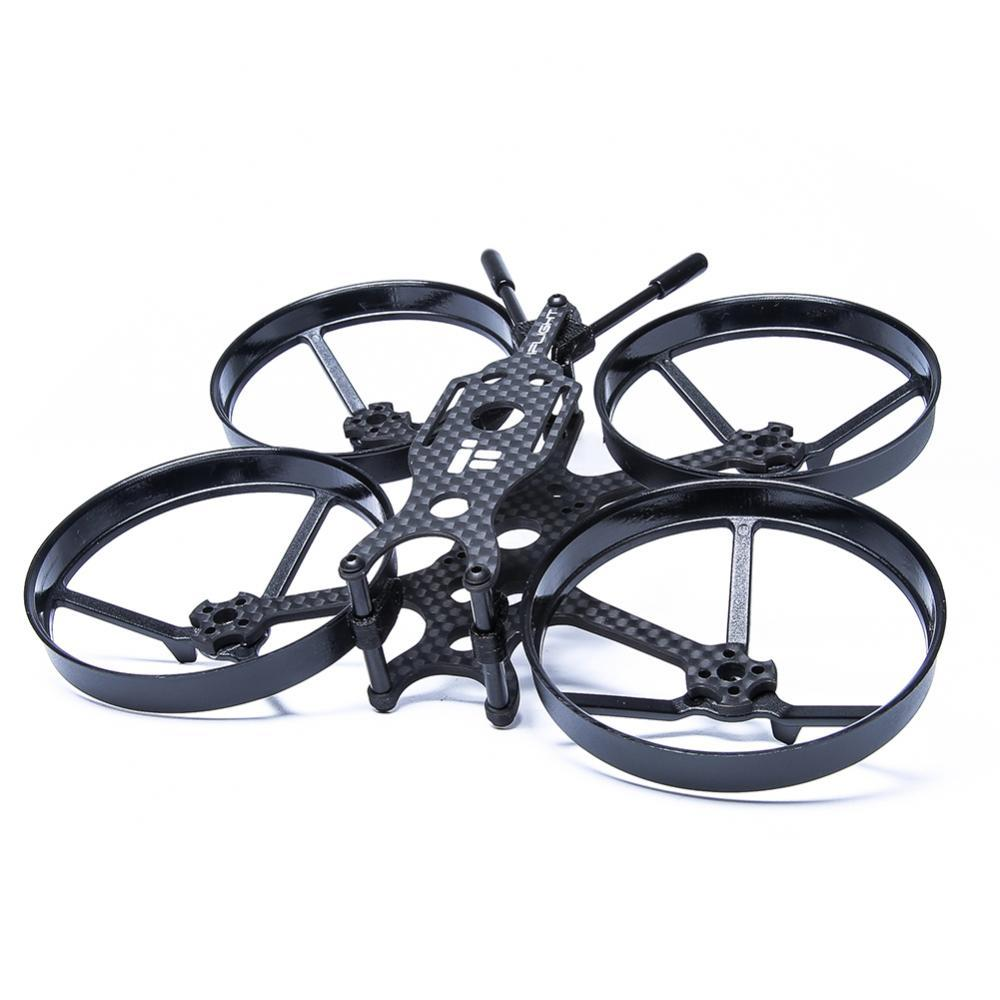
\includegraphics[width=0.5\linewidth]{../RW/pics/frame}
	\caption{Рама для экспериментального образца квадрокоптера
	}
	\label{fig:frame}
\end{figure}

Данная рама используется для создания экспериментального образца. В случае массового производства комплектов, которые будут получены при достижении поставленной цели, рама может быть заменена собственной разработкой.

Перейдем к выбору электроники.

Электроника квадрокоптера должна быть совместимой по характеристикам и габаритам. 

Для управления с наземной станции полетный контроллер должен:
\begin{itemize}
	\item обладать минимум 2 UART портами;
	\item иметь процессор на базе F405 / F745 / F765 чипа.
\end{itemize}
UART (Universal asynchronous receiver/transmitter) -- это аппаратный последовательный интерфейс, который позволяет подключать датчики и периферию к полетному контроллеру. У него есть два вывода для внешнего соединения: TX -- для передачи данных, RX -- для приема.

UART порты потребуются для подключения устройства приема -- передачи телеметрии и возможности подключения дополнительной периферии.

Выбор чипа процессора основан на требованиях к ресурсам по памяти, производительности и периферии. Для того, чтобы прошить PX4, необходим объем памяти процессора не ниже 1 МБ. Такое условие выполняют процессоры на базе F405 / F745 / F765. Преимущество F7 чипов в том, что обеспечивается больше памяти и портов, а также лучше поддерживаются. Но они дороже, выбор полетных контроллеров на таких чипах меньше, а разработка собственного полетного контроллера пока не целесообразна.

Винто -- моторная группа должна быть оптимизирована под задачи автономного полета в помещении на небольшой скорости и устанавливаться в выбранную раму. У моторов бесколлекторного типа основными параметрами являются размеры статора -- неподвижной части мотора (4 цифры) и количество оборотов на вольт(kv). В четырехзначном числе первые два отвечают за диаметр статора, вторые -- за высоту статора. При одинаковых объемах статора крутящий момент на низких оборотах будет больше у того мотора, где больше диаметр статора, а на высоких оборотах там, где больше высота. Для экспериментального образца оптимальным выбором являются моторы 1202. Количество оборотов на вольт выберем, учитывая напряжение аккумулятора. Чем больше напряжение, тем меньше количество оборотов на вольт должно быть на моторе. Каждая ячейка, подключенная последовательно увеличивает напряжение на 4.2 В в заряженном состоянии. Для квадрокоптера с диагональю рамы 120 мм по соотношению вес / токоотдача наиболее выгодно ставить аккумуляторы с 2-3 ячейками. Основываясь на таблице характеристик, приведенных производителем, были выбраны моторы с 6000 kv (рисунок \ref{fig:motor}).
Учитывая потребление тока моторами на полном газу и добавляя 10 -- 15 \% запаса, получаем характеристику регуляторов -- максимальный ток, проходящий через них. На экспериментальном образце он равен 15 А.
\begin{figure}[H]
	\centering
	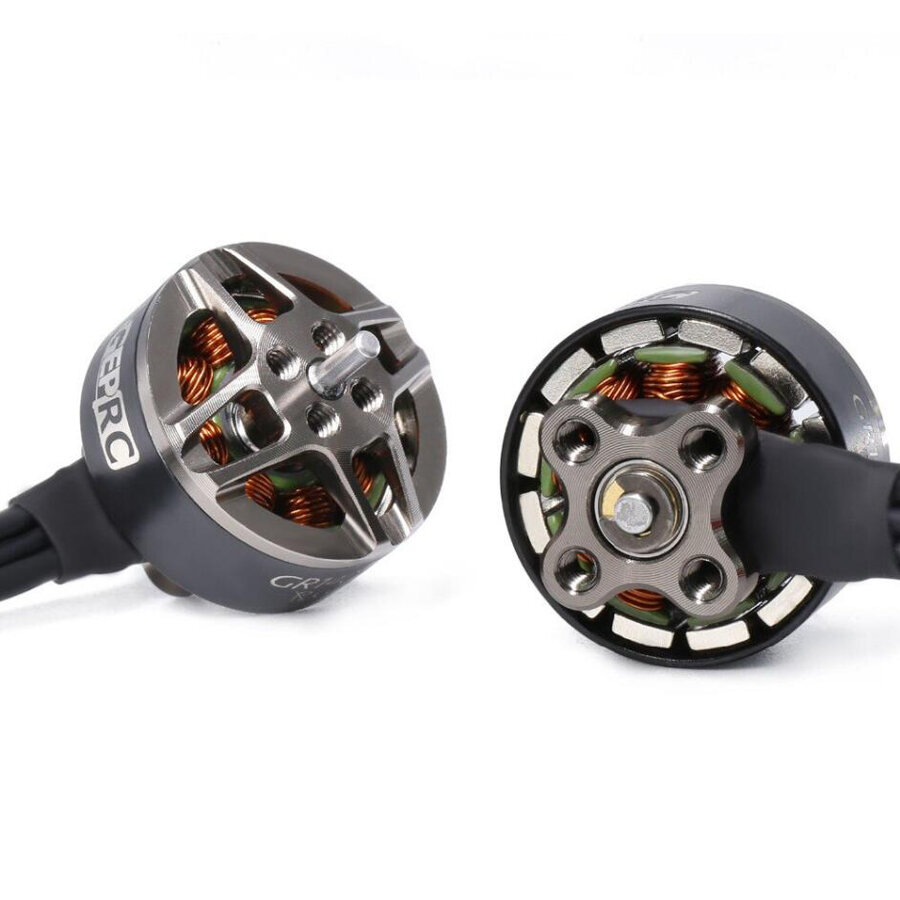
\includegraphics[width=0.5\linewidth]{../RW/pics/motor}
	\caption{Моторы для экспериментального образца квадрокоптера
	}
	\label{fig:motor} % эта метка позволяет ссылаться на рисунок в тексте
\end{figure}
\begin{figure}[H]
	\centering
	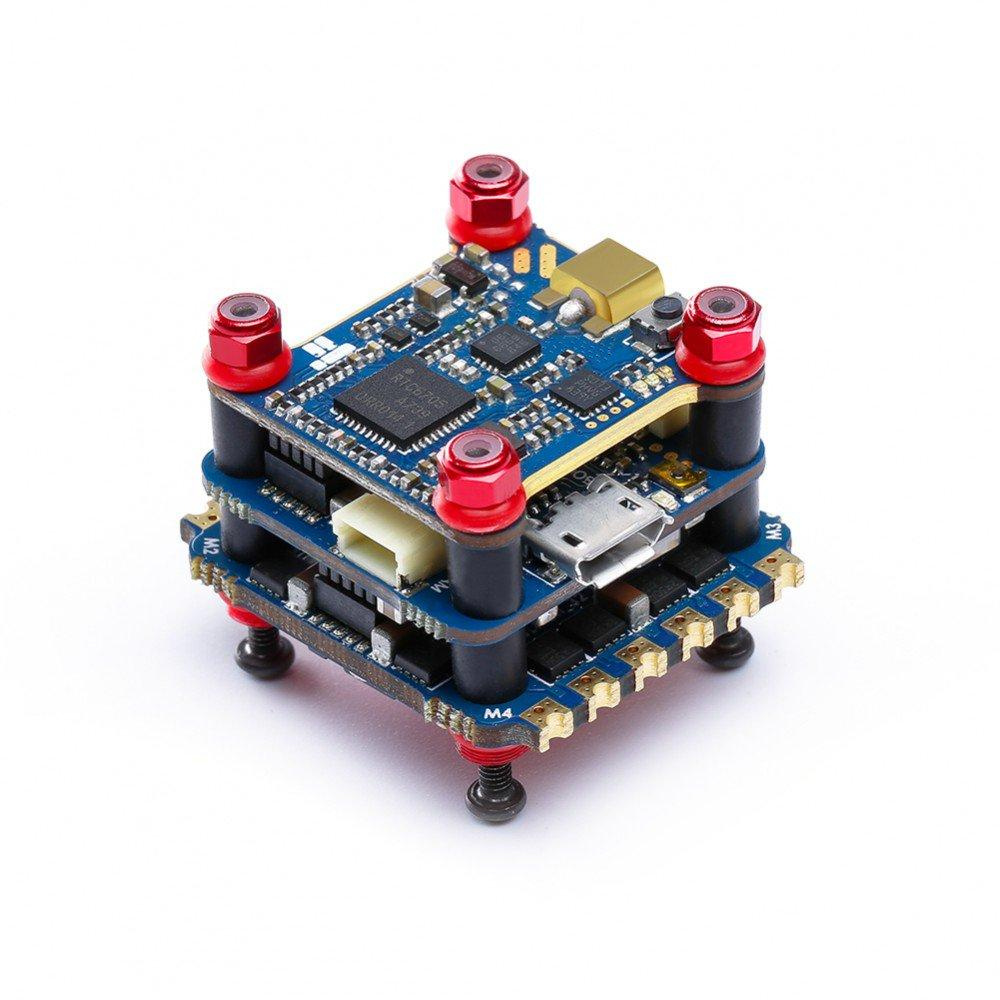
\includegraphics[width=0.5\linewidth]{../RW/pics/stack}
	\caption{Стек электроники для экспериментального образца квадрокоптера
	}
	\label{fig:stack} % эта метка позволяет ссылаться на рисунок в тексте
\end{figure}
Видеопередатчик и камера выбирались исходя из поставленных условий. Видеосигнал аналогового типа дешевле и передается с задержкой меньше, чем цифровой сигнал. MVP решение будем основывать на аналоговом сигнале. Так как необходимо будет передавать видеопоток, камера должна иметь максимально возможное количество телевизионных линий -- разрешающая способность (TVL). Для камер нано формата это 1000 TVL. Размер изображения может быть как 4:3 и 16:9. Формат PAL / NTSC также может быть выбран на усмотрение.

Видеопередатчик обладает такими характеристиками как:
\begin{itemize}
	\item выходная мощность;
	\item выходная частота;
	\item количество каналов.
\end{itemize}
Для помещений мощность 25mW является оптимальной. Количество каналов должно быть выбрано таким образом, чтобы в случае совместных полетов сигнал не пересекался с сигналом другого беспилотника. Современные видеопередатчики имеют 40 каналов. Частота видеосигнала будет использоваться 5.8ГГц.

Для общения с наземной станцией квадрокоптеру понадобятся устройства приема-передачи телеметрии. Протокол, бод-рейт (скорость передачи данных для подключенного устройства приема-передачи данных) и частота устройств станции и квадрокоптера должны совпадать.

Программная часть квадрокоптера полностью осуществляется прошивкой PX4.

%//estimator lpe / ekf
%\url{https://dev.px4.io/v1.9.0/en/ros/offboard\_control.html}
%\url{https://dev.px4.io/v1.9.0/en/ros/external_position_estimation.html}

